\chapter{Testing}

\section{Partita single player}
\begin{figure}[!ht]
	\centering
	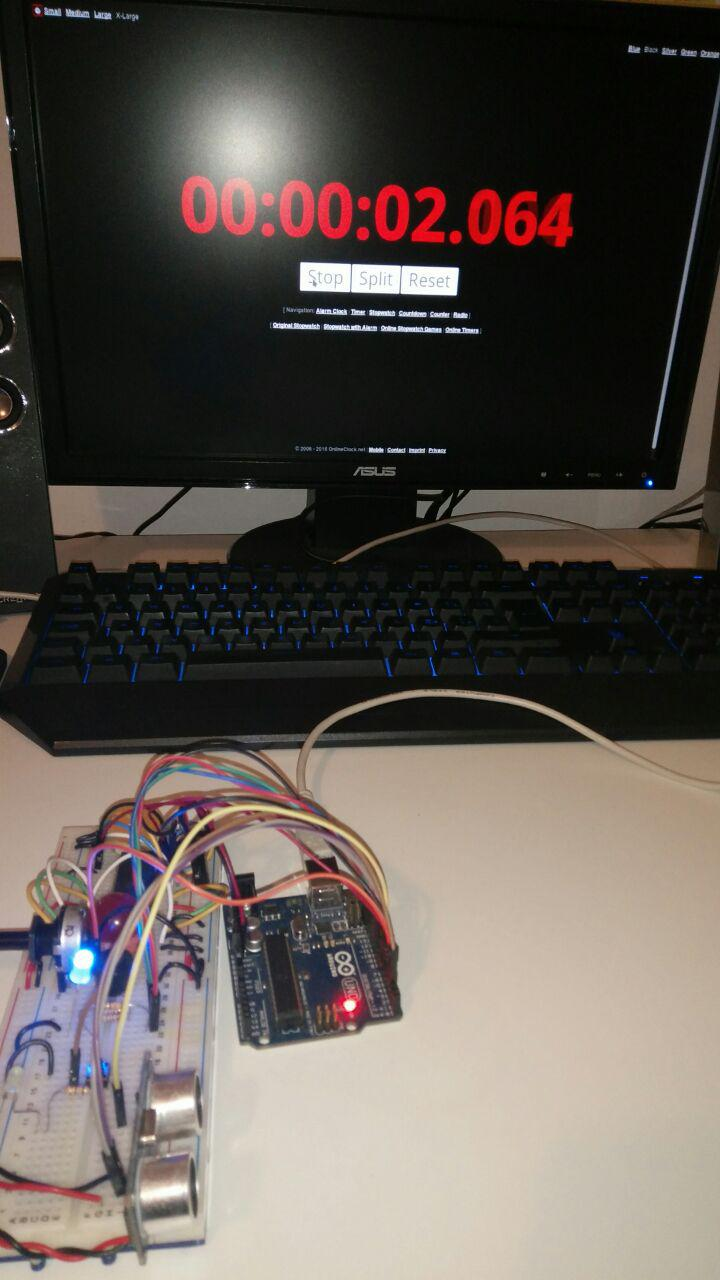
\includegraphics[scale=.25]{img/testing/testing1.jpg}
	\caption{\href{https://youtu.be/X0QOKkfVF4Y}{Testing cronometrato}}
\end{figure}

\clearpage
\section{Web Application}
\subsection{Fase di login}

\begin{figure}[!ht]
	\centering
	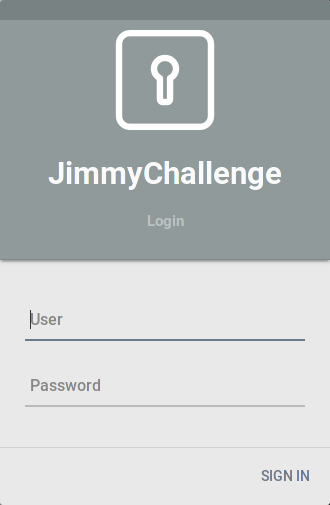
\includegraphics[scale=.4]{img/testing/login.png}
	\caption{Form di login}
\end{figure}

\begin{figure}[!ht]
	\centering
	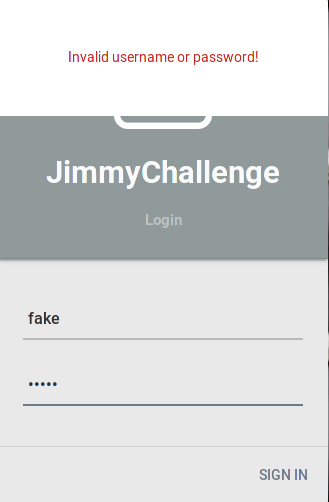
\includegraphics[scale=.4]{img/testing/login_error.png}
	\caption{Errore di login}
\end{figure}

\clearpage
\subsection{Fase di gioco}
\begin{figure}[!ht]
	\centering
	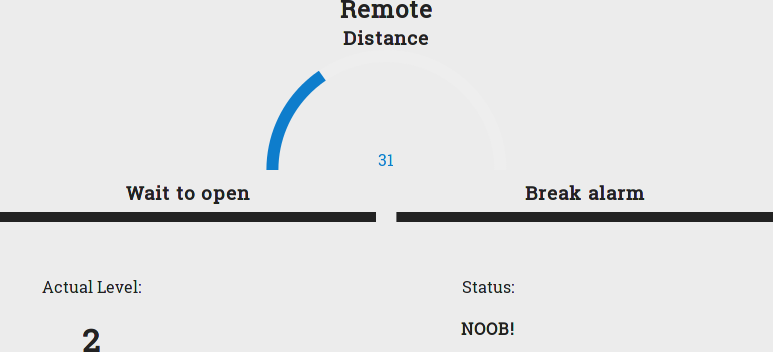
\includegraphics[scale=.4]{img/testing/game1.png}
	\caption{Pistoncino non trovato}
\end{figure}

\begin{figure}[!ht]
	\centering
	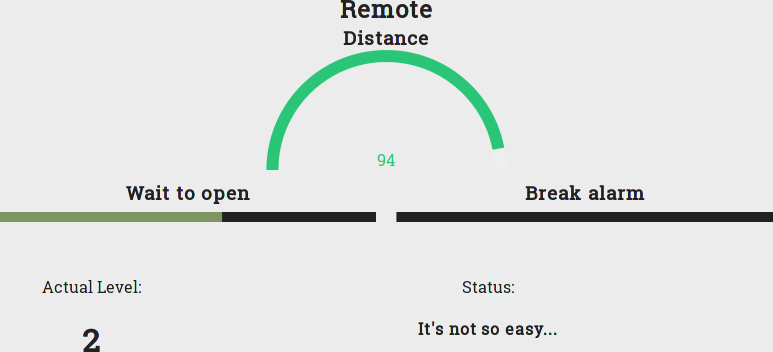
\includegraphics[scale=.4]{img/testing/game2.png}
	\caption{Pistoncino trovato, inizio stato di scasso}
\end{figure}

\begin{figure}[!ht]
	\centering
	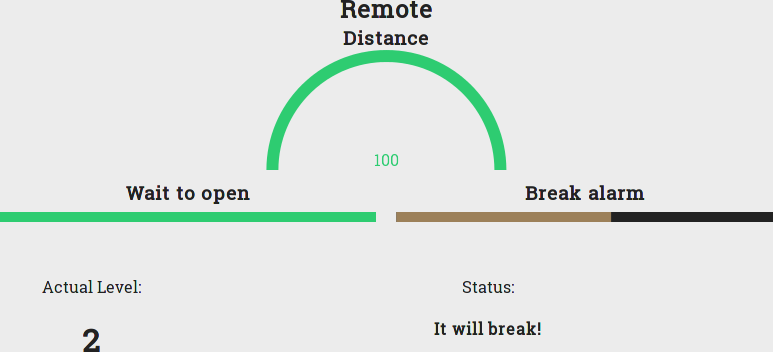
\includegraphics[scale=.4]{img/testing/game3.png}
	\caption{Stato di scasso, rischio rottura}
\end{figure}

\begin{figure}[!ht]
	\centering
	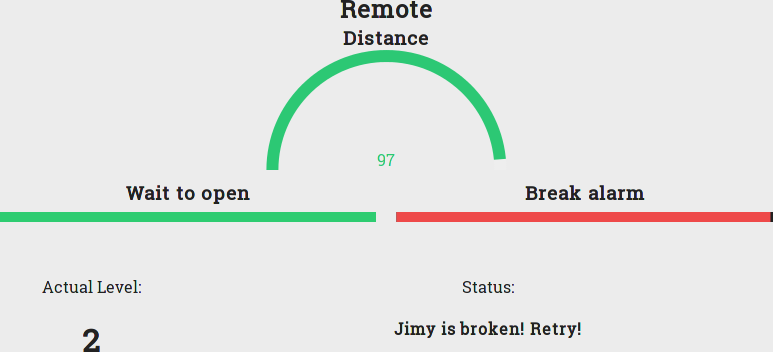
\includegraphics[scale=.4]{img/testing/game4.png}
	\caption{Grimaldello rotto}
\end{figure}

\begin{figure}[!ht]
	\centering
	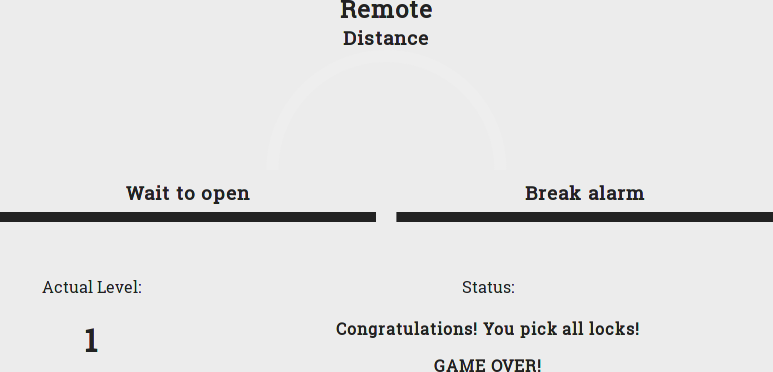
\includegraphics[scale=.4]{img/testing/game5.png}
	\caption{Gioco finito}
\end{figure}

